\subsection{Hadoop}

Hadoop\footnote{https://hadoop.apache.org/} ist ein Projekt von Apache für die verteilte Datenverarbeitung auf einem Cluster.
Die Verarbeitung basiert auf  Map-Reduce \parencite{mapred}, einem Programmier-Modell, bei dem Daten in Form von Schlüssel-Wert-Paaren verarbeitet werden.
Grob beschrieben, besteht es aus zwei Funktionen.
Die erste ist die Map-Funktion, bei der aus Daten eine Zwischensammlung von Schlüssel-Wert-Paaren erzeugt wird.
Danach werden diese nach den Schlüsseln sortiert und die Reduce-Funktion, zum Zusammenfassen der Paare ausgeführt.
Ein Hadoop-Cluster enthält zwei wichtige Komponenten.
YARN \parencite{yarn} wird für das Ressourcen-Management benutzt.
Die zweite Komponente, das HDFS, ist ein verteiltes und fehlertolerantes Dateisystem, welches ursprünglich für Hadoop entwickelt wurde.
Für dieses Projekt ist nur das HDFS relevant und wird deswegen näher erläutert.

Das HDFS wurde entwickelt, um auf Hardware mit geringen Kosten zu laufen und große Datenmengen zu verarbeiten.
Dateien können von einem Gigabyte bis mehrere Terabyte groß sein.
Die Fehlertoleranz wird dabei durch die Möglichkeit der Replikation mit einem beliebigen Faktor gegeben.

Das Dateisystem ist ähnlich zu anderen bekannten Dateisystemen aufgebaut.
Dateien und Ordner können im Namensraum hierarchisch organisiert werden.
Es unterstützt jedoch keine Zugriffsberechtigung oder Hard- und Soft-Links.
Um einfach und effektiv kohärent zu bleiben, werden Dateien nur einmal geschrieben, können aber mehrfach gelesen werden.
Dateien werden zur Speicherung in einzelne Blöcke aufgeteilt.
Dabei sind für eine Datei alle Blöcke, bis auf den letzten, gleich groß.

\begin{figure}
    \centering
    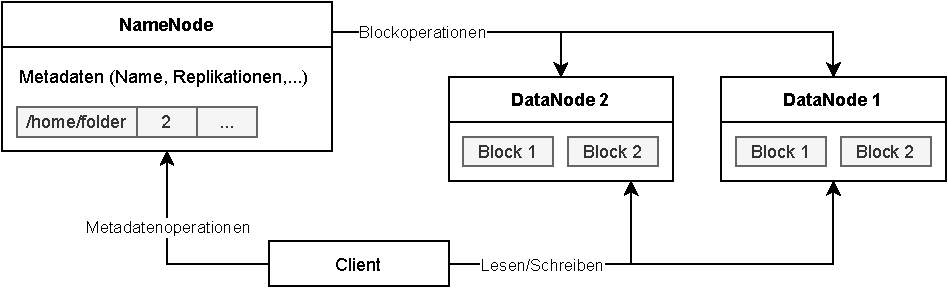
\includegraphics[width=\textwidth]{Grafiken/Grundlagen/HDFS.pdf}
    \caption[HDFS-Architektur]{HDFS-Architektur\footnotemark}
    \label{fig:hdfs-cluster}
\end{figure}
\footnotetext{Nach https://hadoop.apache.org/docs/r1.2.1/images/hdfsarchitecture.gif, Zugriff: 29.12.2021}

Ein HDFS-Cluster (\cref{fig:hdfs-cluster}) funktioniert nach dem Master-Worker-Prinzip und besteht aus einem NameNode und vielen DataNodes.
Der NameNode übernimmt die Verwaltung des Namensraums und die Verteilung der einzelnen Blöcke einer Datei.
Er reguliert dazu noch den Zugriff durch Clients und führt Operationen auf dem Dateisystem, wie das Öffnen, Schließen oder Umbenennen von Ordnern und Dateien aus.
Die DataNodes speichern die einzelnen Blöcke der Dateien.
Auf Anweisung des NameNode werden Blöcke erstellt, gelöscht oder repliziert.
Außerdem bearbeiten sie Anfragen zum Lesen und Schreiben von Dateien \parencite{hdfs}.

% Parquet
Mit Apache Parquet steht ein Format zur Verfügung, mit dem Daten im HDFS effizient gespeichert werden können.
Parquet ist ein spalten-orientiertes Speicherformat, das auch die Kompression und Kodierung der Daten unterstützt.
Über einen Algorithmus zur Zerlegung von Verschachtelung ist auch das Speichern von semistrukturierten Daten möglich \parencite{parquet}.
